\documentclass[11pt]{beamer}
\let\Tiny=\tiny

\usefonttheme[onlymath]{serif}

\usepackage{color}
\usepackage{colortbl}
\usepackage{multicol}
\usepackage{amssymb,amsmath,amsthm,stmaryrd}
\usepackage{indentfirst}
\usepackage{latexsym}
\usepackage[utf8]{inputenc}
\usepackage{fancybox}
\usepackage{tikz}
\usepackage{tikz-qtree}
\usepackage{eurosym}
\usepackage{listings}
\usepackage{soul}
\usepackage{upquote}
\usepackage{cancel}
\usepackage{xfrac}

\definecolor{light_red}{rgb}{1,0.95,0.95} 
\definecolor{gray}{rgb}{0.5,0.5,0.5} 
\definecolor{green}{rgb}{0.05,0.4,0.25} 

\usetikzlibrary{trees,shapes,decorations}

\setbeamertemplate{navigation symbols}{}
\setbeamercovered{transparent}

\title[Lekta framework practical tutorial]{Lekta framework practical tutorial}
\author{Jose F Quesada \& Jose Luis Pro}
\date{}

\mode<presentation>{\usetheme[]{Warsaw}}

\setbeamertemplate{footline}
    {
      \leavevmode
      \hbox{\begin{beamercolorbox}[wd=.5\paperwidth,ht=2.5ex,dp=1.125ex,leftskip=.3cm plus1fill,rightskip=.3cm]{author in head/foot}
        \usebeamerfont{author in head/foot}\insertshorttitle%
      \end{beamercolorbox}%
      \begin{beamercolorbox}[wd=.5\paperwidth,ht=2.5ex,dp=1.125ex,leftskip=.3cm,rightskip=.3cm plus1fil]{title in head/foot}
        \usebeamerfont{title in head/foot}
					\hfill\insertframenumber\,/\,\inserttotalframenumber
      \end{beamercolorbox}}
      \vskip0pt
    }

\hypersetup{pdfpagemode=UseNone}

\newcommand{\Operator}[1]{\textcolor{green}{#1}}

\lstset
{
	basicstyle=\ttfamily,
	keywordstyle=\color{blue}\ttfamily,
  stringstyle=\color{red}\ttfamily,
  commentstyle=\color{green}\ttfamily,
  language=C,                			% choose the language of the code
  numbers=left,                   % where to put the line-numbers
  stepnumber=1,                   % the step between two line-numbers.        
  numbersep=5pt,                  % how far the line-numbers are from the code
  backgroundcolor=\color{white},  % choose the background color. You must add \usepackage{color}
  showspaces=false,               % show spaces adding particular underscores
  showstringspaces=false,         % underline spaces within strings
  showtabs=false,                 % show tabs within strings adding particular underscores
  tabsize=3,                      % sets default tabsize to 3 spaces
  captionpos=b,                   % sets the caption-position to bottom
  breaklines=true,                % sets automatic line breaking
  breakatwhitespace=true,         % sets if automatic breaks should only happen at whitespace
}

\lstdefinelanguage{lekta}
{
	language=C,
	backgroundcolor=\color{light_red},
	numberstyle=\tiny\color{gray},
	morekeywords=
	{
		classDef,
		Void,
		cond,
		boolean,
		String,
		True,
		False,
		\#Include,
	},
	alsoletter={\#},
	literate= {->}{{\Operator{->}}}1
						{>>}{{\Operator{>>}}}1
						{\&\&}{{\Operator{\&\&}}}1
						,	
	keywordstyle=[2]\color{purple},
	keywords=[2]
	{
		lektaProject,
		projectHead,
		projectLanguageScope,
		projectCompileOutput,
		projectSetup,
		setupParserRoots,
		classModel,
		lexicalModel,
		forLanguage,
		grammaticalModel,
		LaunchLektaKernel,
		UseProject,
		ProjectCompile,
		DisplayProcessUnderstandingOn,
		CreateDialogue,
		ElementBool,
		ElementInt,
		ElementReal,
		ElementLiteral,
		ElementRange,
		StructureBatch,
		StructureComplex,
		Synonym,
		MindBoardStructure,
		conversationalModel,
		ColligoSchemata,
		ColligoCapture,
		ColligoScheme,
		ColligoAction,
		SensoSchemata,
		SensoScheme,
		SensoCapture,
		SensoAction,
		CogitoScheme,
		CogitoCapture,
		CogitoAction,
		CogitoSchemata,
		RespondoSchemata,
		RespondoScheme,
		RespondoCapture,
		RespondoAction,
		LocutioSchemata,
		LocutioScheme,
		LocutioCapture,
		LocutioAction,
		scriboModel,
		ScriboSchemata,
		ScriboScheme,
		ScriboCapture,
		ScriboAction,
	},
}

\begin{document}

\begin{frame}
\titlepage
\end{frame}

\section{Session 01: Formal languages}

\subsection{Exercise 01}

\begin{frame}
	\setbeamercolor{block title}{use=structure,fg=white,bg=red!75!black}
	\setbeamercolor{block body}{use=structure,fg=black,bg=red!10!white}
	\begin{block}{What is Lekta?}
			Lekta is a software \textbf{framework} oriented to the design and implementation of Natural Language Processing (NLP) related applications. This includes:
			\pause
			\begin{itemize}
				\item Some specialized and \textbf{optimized} modules widely used in NLP applications (tokenizer, parser and so on). You'll never reinvent the wheel anymore.
				\pause
				\item A simple and efficient way to define lexicons and grammar rules for any language.
				\pause
				\item Early multilingual support for all your applications.
				\pause
				\item A set of built-in functions that you'll find useful when implementing your NLP oriented app.
				\pause
				\item A programming language to interact with all items above and to define your own functions or procedures.
			\end{itemize}
	\end{block}
\end{frame}

\begin{frame}[fragile]
\frametitle{Basic project setup}
A lekta project is composed of a single text file.\\
\vspace{5pt}
\pause
This file starts with the keyword ``\texttt{lektaProject}'' and has, at least, five sections:
\vspace{5pt}
\pause
\scriptsize
\begin{lstlisting}[language=lekta]
lektaProject

	projectHead
		<...>

	projectSetup
		<...>
		
	classModel
		<...>

	lexicalModel forLanguage <...>
		<...>
		
	grammaticalModel forLanguage <...>
		<...>

\end{lstlisting}
\end{frame}

\begin{frame}[fragile]
\frametitle{AnBm.lkt (1/4)}
	\setbeamercolor{block title}{use=structure,fg=white,bg=green!75!black}
	\setbeamercolor{block body}{use=structure,fg=black,bg=green!10!white}
	\begin{block}{Example}
			\begin{itemize}
				\item We would like to create a very simple lekta project.
				\pause
				\item It must be able to recognize sentences in a formal language defined as $A_nB_m$ with $n,m \geq 1$. 
				\pause
				\item In other words, this language is composed by all the strings that have at least one ``a'' followed by, at least, one ``b''.
				\pause
				\item \texttt{a a a a b b b}: {\color{green}Correct}.
				\pause
				\item \texttt{b b b a a a a}: {\color{red}Incorrect}.
			\end{itemize}
	\end{block}
\pause
\scriptsize
\begin{lstlisting}[language=lekta]
projectHead
	// Languages defined for this project.
	projectLanguageScope : [ anbm ]
	
	// Output file after compiling.
	projectCompileOutput : ".AnBm.olk"
\end{lstlisting}
\end{frame}

\begin{frame}[fragile]
\frametitle{AnBm.lkt (2/4)}
\small
\begin{lstlisting}[language=lekta]
projectSetup
	// Possible output parser types.
	setupParserRoots = S

classModel
	// Definition of all the types needed.
	// Type Void acts as a label.
	classDef:Void ( S, A, B, a, b )

// Lexical model is language dependant
lexicalModel forLanguage anbm
	// Lexicon elements that we must detect.
	// Here a and b act as grammar terminal symbols.
	("a", a)
	("b", b)
\end{lstlisting}
\end{frame}

\begin{frame}[fragile]
\frametitle{AnBm.lkt (3/4)}
\begin{lstlisting}[language=lekta]
// Grammatical model is language dependant
grammaticalModel forLanguage anbm
	// List of grammar rules 
	/* Always context free grammar. Among other things, this means that left part of the rule must be composed by one and only one non-terminal symbol */
	(R1: [ S -> a A b B ])
	(R2: [ A -> ])
	(R3: [ A -> a A ])
	(R4: [ B -> ])
	(R5: [ B -> b B ])
\end{lstlisting}
\end{frame}

\begin{frame}[fragile]
\frametitle{AnBm.lkt (4/4)}
\tiny
\begin{lstlisting}[language=lekta]
// *********************************************************************
//
// Exercise 01: Generator/Recognizer for language AnBm. Where n,m >= 1
//
// *********************************************************************

lektaProject
	projectHead
		projectLanguageScope : [ anbm ]
		projectCompileOutput : ".AnBm.olk"

	projectSetup
		setupParserRoots = S

	classModel
		classDef:Void ( S, A, B, a, b )

	lexicalModel forLanguage anbm
		("a", a)
		("b", b)

	grammaticalModel forLanguage anbm
		(R1: [ S -> a A b B ])
		(R2: [ A -> ])
		(R3: [ A -> a A ])
		(R4: [ B -> ])
		(R5: [ B -> b B ])
\end{lstlisting}
\end{frame}

\begin{frame}[fragile]
\frametitle{Compiling and executing}
\begin{itemize}
	\item After creating \texttt{AnBm.lkt} file we must compile it:
	\pause
	\item \texttt{\$> lektac AnBm.lkt}
	\pause
	\item You must see: ``\texttt{Compilation Succesfully Finished}'' message.
	\pause
	\item And after that you must create a file for the lekta interpreter, \texttt{AnBm.slk}, to test and execute the project:
	\pause
	\item \texttt{\$> synclekta AnBm.slk}
\end{itemize}
\tiny
\begin{lstlisting}[language=lekta]
// Start lekta engine
LaunchLektaKernel()

// Use recently compiled project
UseProject (ProjectCompile : ".AnBm.olk")

// Options for visualization
DisplayProcessUnderstandingOn

// Start a dialogue with lekta
CreateDialogue()
\end{lstlisting}
\end{frame}

\begin{frame}[fragile]
\Huge
\begin{center}
Session 01: Exercise 01\\
AnBm
\end{center}
\end{frame}

\subsection{Exercise 02}

\begin{frame}[fragile]
\frametitle{Grammar rules syntax}
\begin{lstlisting}[language=lekta]
(<rule_label>:
	[ <symbol> -> <list_of_symbols> ]
	{
		...
		<commands>
		...
	}
)
\end{lstlisting}
\pause
\begin{itemize}
	\item \texttt{<rule\_label>} Only useful for readability and debugging.
	\item \texttt{<symbol>} A non-terminal symbol.
	\item \texttt{<list\_of\_symbols>} List of terminal and non-terminal symbols needed for the triggering of this rule.
	\item \texttt{<commands>} Commands to be executed  when this rule is triggered.
\end{itemize}
\end{frame}

\begin{frame}[fragile]
\frametitle{Special features: Optional symbol (?)}
\small
Rule \texttt{R2} can be interpreted as a mandatory `a' followed (or not) by `A'.
\begin{lstlisting}[language=lekta]
(R1: [ S -> A? B? ])
(R2: [ A -> a A? ])
\end{lstlisting}
\pause
\begin{lstlisting}[language=lekta]
// These rules are expanded into standard rules
(R1: [ S -> A B ])
(R1: [ S -> B ])
(R1: [ S -> A ])
(R1: [ S -> ])

(R2: [ A -> a A ])
(R2: [ A -> a ])
\end{lstlisting}
\end{frame}

\begin{frame}[fragile]
\frametitle{Special features: Or symbol ($|$)}
\small
Rule \texttt{R1} can be interpreted as a mandatory `A' followed by `B', `C' or `D'.
\begin{lstlisting}[language=lekta]
(R1: [ S -> A < B | C | D > ])
\end{lstlisting}
\pause
\begin{lstlisting}[language=lekta]
// These rules are expanded into standard rules
(R1: [ S -> A B ])
(R1: [ S -> A C ])
(R1: [ S -> A D ])
\end{lstlisting}
\vspace{15pt}
\pause
Special symbols can be combined:
\begin{lstlisting}[language=lekta]
(R1: [ S -> A < B | C >? ])

(R1: [ S -> A ])
(R1: [ S -> A B ])
(R1: [ S -> A C ])
\end{lstlisting}
\end{frame}

\begin{frame}[fragile]
\frametitle{Special features: Free order symbol (\%)}
\small
Rule \texttt{R1} can be interpreted as a mandatory `A' followed by `B', `C' and `D' in any order.
\begin{lstlisting}[language=lekta]
(R1: [ S -> A < B % C % D > ])
\end{lstlisting}
\pause
\begin{lstlisting}[language=lekta]
// These rules are expanded into standard rules
(R1: [ S -> A B C D ])
(R1: [ S -> A B D C ])
(R1: [ S -> A C B D ])
(R1: [ S -> A C D B ])
(R1: [ S -> A D B C ])
(R1: [ S -> A D C B ])
\end{lstlisting}
\vspace{10pt}
\pause
When combining several special symbols we must take into account exponentially growing in the number of rules.
\begin{lstlisting}[language=lekta]
// 12 Rules when expanding
(R1: [ S -> A < B % C % < D | E > > ])
\end{lstlisting}
\end{frame}

\begin{frame}[fragile]
\frametitle{Special features: Left and right limits (\&[+\^{}] and [+\$]\&)}
\small
Rule \texttt{R1} will only be triggered if there is nothing to the left of `A' expression:
\begin{lstlisting}[language=lekta]
(R1: [ S -> &[+^] A B ])
\end{lstlisting}
\pause
\vspace{15pt}
Rule \texttt{R1} will only be triggered if there is nothing to the right of `B' expression:
\begin{lstlisting}[language=lekta]
(R1: [ S -> A B [+$]& ])
\end{lstlisting}
\pause
\vspace{15pt}
Rule \texttt{R1} will only be triggered if there is nothing to the left of `A' expression and nothing to the right of `B' expression:
\begin{lstlisting}[language=lekta]
(R1: [ S -> &[+^] A B [+$]& ])
\end{lstlisting}
\end{frame}

\begin{frame}[fragile]
\Huge
\begin{center}
Session 01: Exercise 02\\
AnBm with optional parameters
\end{center}
\end{frame}

\subsection{Exercise 03}

\begin{frame}[fragile]
\Huge
\begin{center}
Session 01: Exercise 03\\
AnBmCn
\end{center}
\end{frame}

\subsection{Exercise 04}

\begin{frame}[fragile]
\frametitle{Type specification in Lekta}
\begin{itemize}
	\item At the very beginning we have not any type in our project.
	\pause
	\item So you must create all the types you may need (with \texttt{classDef} keyword).
	\pause
	\item To create new types we have metatypes (or type creators) in Lekta:
	\begin{enumerate}
		\item \texttt{ElementBool}: Boolean metatype.
		\item \texttt{ElementInt}: Integer numbers metatype.
		\item \texttt{ElementReal}: Real numbers metatype.
		\item \texttt{ElementLiteral}: Strings of characters.
		\item \texttt{ElementMessage}: Messages.
		\item \texttt{ElementRange}: Enumerate type.
		\item \texttt{StructureBatch}: Sequence of elements of the same type.
		\item \texttt{StructureComplex}: Structure of elements of any type.
	\end{enumerate}
\end{itemize}
\end{frame}

\begin{frame}[fragile]
\frametitle{Type specification in Lekta}
\begin{itemize}
	\item So you \textbf{can't} declare a variable of type \texttt{ElementInt}.	
	\pause
	\item But you \textbf{can} create a type (let's say ``\texttt{integer}'') with the metatype \texttt{ElementInt} and declare a variable of type \texttt{integer}.
\end{itemize}
\pause
\setbeamercolor{block title}{use=structure,fg=white,bg=red!75!black}
\setbeamercolor{block body}{use=structure,fg=black,bg=red!10!white}
\begin{block}{Incorrect Example}
\scriptsize
\begin{lstlisting}[language=lekta]
...
ElementInt i <- 5; 
...
\end{lstlisting}
\end{block}
\pause
\setbeamercolor{block title}{use=structure,fg=white,bg=green!75!black}
\setbeamercolor{block body}{use=structure,fg=black,bg=green!10!white}
\begin{block}{Correct Example}
\scriptsize
\begin{lstlisting}[language=lekta]
classDef:ElementInt ( integer )
...
integer i <- 5;
...
\end{lstlisting}
\end{block}
\end{frame}

\begin{frame}[fragile]
\frametitle{Type specification in Lekta}
\begin{itemize}
	\item Sometimes is useful to create some basic types in the beginning.
	\pause
	\item For example, if you are Java fan:
\end{itemize}
\begin{lstlisting}[language=lekta]
classDef:ElementInt     ( int ) 
classDef:ElementBool    ( boolean ) 
classDef:ElementLiteral ( String )
...
int i <- 5; 
boolean flag <- False;
String s <- 'this is a string';
...
\end{lstlisting}
\end{frame}

\begin{frame}[fragile]
\frametitle{Complex structures}
\footnotesize
\begin{lstlisting}[language=lekta]
classDef:ElementInt     (Counter)
classDef:ElementBool    (Flag)
classDef:ElementLiteral (Expression)
classDef:StructureComplex 
( 
	ExampleStructure:
	(
		Counter,
		Flag,
		Expression
	)
)
...
ExampleStructure a;
a.Counter <- 5;
a.Flag <- True;
a.Expression <- 'this is a string';
...
\end{lstlisting}
\end{frame}

\begin{frame}[fragile]
\begin{itemize}
	\item Previous exercises only make some syntactic analysis of the language.
	\pause
	\item So we can only recognize valid sentences in that language (paser output is a void `\texttt{S}').
	\pause
	\item But we want now to do different things with that sentences.
	\pause
	\item So, how can we provide some semantic content to \texttt{AnBm} language?
	\pause
	\item The only reasonable semantic content is to have `\texttt{n}' and `\texttt{m}' values associated with `\texttt{S}' structure.
\end{itemize}
\footnotesize
\begin{lstlisting}[language=lekta]
classDef:ElementInt ( counterN, counterM )
classDef:StructureComplex ( S:( counterN, counterM ) )
classDef:StructureComplex ( A:( counterN ) )
classDef:StructureComplex ( B:( counterM ) )
classDef:Void ( a, b )
\end{lstlisting}
\end{frame}

\begin{frame}[fragile]
\scriptsize
\begin{lstlisting}[language=lekta]
(R1: [ S -> A B ] {
		^.counterN <- #1.counterN;
		^.counterM <- #2.counterM; } )

(R2: [ A -> a A ] {
		^.counterN <- 1 + #2.counterN; } )

(R3: [ A -> a ] {
		^.counterN <- 1; } )

(R4: [ B -> b B ] {
		^.counterM <- 1 + #2.counterM; } )

(R5: [ B -> b ] {
		^.counterM <- 1; } )
\end{lstlisting}
\footnotesize
Note special syntax:
\begin{itemize}
	\item \texttt{\^{}} stands for left side term generated by the rule (upper node in parsing tree).
	\item \texttt{\#1} stands for the first term in the right side of the rule.
	\item \texttt{\#2} stands for the second term in the right side of the rule.
	\item \texttt{\#N} stands for the nth term in the right side of the rule.
\end{itemize}
\end{frame}

\begin{frame}[fragile]
\Huge
\begin{center}
Session 01: Exercise 04\\
AnBn
\end{center}
\end{frame}

\section{Session 02: Natural language}

\subsection{Exercise 01}

\begin{frame}[fragile]
\Huge
\begin{center}
Session 02: Exercise 01\\
English lexicon and grammar
\end{center}
\end{frame}

\subsection{Exercise 02}

\begin{frame}[fragile]
\frametitle{Files inclusion}
\footnotesize
\begin{lstlisting}[language=lekta]
lektaProject
	
	projectHead
		projectLanguageScope	: [ en ]
		projectCompileOutput	: ".Numbers.olk"

	projectSetup
		setupParserRoots = Number

	classModel
		#Include "NumberTypes.lkt"

	lexicalModel forLanguage en
		#Include "NumberEnglishLexicon.lkt"

	grammaticalModel forLanguage en
		#Include "NumberEnglishGrammar.lkt"
\end{lstlisting}
\end{frame}

\begin{frame}[fragile]
\setbeamercolor{block title}{use=structure,fg=white,bg=green!75!black}
\setbeamercolor{block body}{use=structure,fg=black,bg=green!10!white}
\begin{block}{Function and procedure declaration}
\scriptsize
\begin{lstlisting}[language=lekta]
classDef:ElementInt ( integer )
classDef:ElementBool ( bool )
// Templates
<ouput_type> function_name(<parameter_list>) {
	...
}
procedure function_name(<parameter_list>) {
	...
}

// Examples
bool f1(integer i) {
	...
}
procedure f2(integer i) {
	...
}
procedure f3() { // Not "void" keyword
	...
}
\end{lstlisting}
\end{block}
\end{frame}

\begin{frame}[fragile]
\setbeamercolor{block title}{use=structure,fg=white,bg=green!75!black}
\setbeamercolor{block body}{use=structure,fg=black,bg=green!10!white}
\begin{block}{Comments}
\small
\begin{lstlisting}[language=lekta]
// This is a mono-line comment
/*	This is a multi-line comment
		with some commented lines	*/
\end{lstlisting}
\end{block}
\pause
\setbeamercolor{block title}{use=structure,fg=white,bg=green!75!black}
\setbeamercolor{block body}{use=structure,fg=black,bg=green!10!white}
\begin{block}{Arithmetic operators}
\begin{lstlisting}[language=lekta]
a <- b + c; // Addition
a <- b - c; // Subtraction
a <- b * c; // Multiplication
a <- b / c; // Division
a++;        // Post-autoincrement
++a;        // Pre-autoincrement
a--;        // Post-autodecrement
--a;        // Pre-autodecrement
\end{lstlisting}
\end{block}
\end{frame}

\begin{frame}[fragile]
\setbeamercolor{block title}{use=structure,fg=white,bg=green!75!black}
\setbeamercolor{block body}{use=structure,fg=black,bg=green!10!white}
\begin{block}{Comparation operators}
\begin{lstlisting}[language=lekta]
a >  b  // Greater
a >= b  // Greater or equal
a <  b  // Less
a <= b  // Less or equal
a == b  // Equal
a != b  // Not equal
\end{lstlisting}
\end{block}
\pause
\setbeamercolor{block title}{use=structure,fg=white,bg=green!75!black}
\setbeamercolor{block body}{use=structure,fg=black,bg=green!10!white}
\begin{block}{Boolean operators}
\begin{lstlisting}[language=lekta]
a && b  // And
a || b  // Or
!! a    // Not
\end{lstlisting}
\end{block}
\end{frame}

\begin{frame}[fragile]
\frametitle{Lazy evaluation}
\scriptsize
\begin{lstlisting}[language=lekta]
boolean f1() 
{
	// Writes a message to standard output
	SpyMessage("Message from f1"); 
	return False;
}

boolean f2() 
{
	SpyMessage("Message from f2"); 
	return True;
}

procedure testingLazyEvaluation() 
{
	boolean b;
	
	b <- f1() && f2(); // "Message from f1"
	b <- f2() || f1(); // "Message from f2"
}
\end{lstlisting}
\end{frame}

\begin{frame}[fragile]
\frametitle{Programming structures: if...else if...else}
\small
\begin{lstlisting}[language=lekta]
if(month == 1)       { ret <- 'January';   }
else if(month == 2)  { ret <- 'February';  }
else if(month == 3)  { ret <- 'March';     }
else if(month == 4)  { ret <- 'April';     }
else if(month == 5)  { ret <- 'May';       }
else if(month == 6)  { ret <- 'June';      }
else if(month == 7)  { ret <- 'July';      }
else if(month == 8)  { ret <- 'August';    }
else if(month == 9)  { ret <- 'September'; }
else if(month == 10) { ret <- 'October';   }
else if(month == 11) { ret <- 'November';  }
else                 { ret <- 'December';  }
\end{lstlisting}
\end{frame}

\begin{frame}[fragile]
\frametitle{Programming structures: switch}
\small
\begin{lstlisting}[language=lekta]
switch (month) 
{
	case  1 { ret <- 'January';}
	case  2 { ret <- 'February';}
	case  3 { ret <- 'March';}
	case  4 { ret <- 'April';}
	case  5 { ret <- 'May';}
	case  6 { ret <- 'June';}
	case  7 { ret <- 'July';}
	case  8 { ret <- 'August';}
	case  9 { ret <- 'September';}
	case 10 { ret <- 'October';}
	case 11 { ret <- 'November';}
	default { ret <- 'December';}
}
\end{lstlisting}
\end{frame}

\begin{frame}[fragile]
\frametitle{Programming structures: cond}
\small
\begin{lstlisting}[language=lekta]
cond
{
	(month == 1)  { ret <- 'January';   }
	(month == 2)  { ret <- 'February';  }
	(month == 3)  { ret <- 'March';     }
	(month == 4)  { ret <- 'April';     }
	(month == 5)  { ret <- 'May';       }
	(month == 6)  { ret <- 'June';      }
	(month == 7)  { ret <- 'July';      }
	(month == 8)  { ret <- 'August';    }
	(month == 9)  { ret <- 'September'; }
	(month == 10) { ret <- 'October';   }
	(month == 11) { ret <- 'November';  }
	default       { ret <- 'December';  }
}
\end{lstlisting}
\end{frame}

\begin{frame}[fragile]
\frametitle{Programming structures: loops}
\setbeamercolor{block title}{use=structure,fg=white,bg=green!75!black}
\setbeamercolor{block body}{use=structure,fg=black,bg=green!10!white}
\begin{block}{``While'' loop}
\scriptsize
\begin{lstlisting}[language=lekta]
integer position,size;
...
position <- 1;
while (position <= size) {
	<...>
	position++;
}
\end{lstlisting}
\end{block}
\pause
\setbeamercolor{block title}{use=structure,fg=white,bg=green!75!black}
\setbeamercolor{block body}{use=structure,fg=black,bg=green!10!white}
\begin{block}{``For'' loop}
\scriptsize
\begin{lstlisting}[language=lekta]
integer position,size;
...
for (position <- 1; position <= size; position++) {
	<...>
}
\end{lstlisting}
\end{block}
\end{frame}

\begin{frame}[fragile]
\frametitle{Built-in functions}
\setbeamercolor{block title}{use=structure,fg=white,bg=green!75!black}
\setbeamercolor{block body}{use=structure,fg=black,bg=green!10!white}
\begin{block}{Mathematics}
\scriptsize
\begin{lstlisting}[language=lekta]
integer Max(integer n1, integer n2);
integer Min(integer n1, integer n2);
integer Ceiling(real r);
integer Floor(real r);
integer Round(real r);
integer Abs(integer n);
integer Modulo(integer dividend, integer divisor);
real Sqrt(real r);
real Pow(real r);
real Exp(real r);
real Log10(real r);
real LogN(real r);
real Sin(real r);
real Cos(real r);
real Tan(real);
integer Random(integer from, integer to);
\end{lstlisting}
\end{block}
\end{frame}

\begin{frame}[fragile]
\frametitle{Built-in functions}
\setbeamercolor{block title}{use=structure,fg=white,bg=green!75!black}
\setbeamercolor{block body}{use=structure,fg=black,bg=green!10!white}
\begin{block}{Date \& time}
\scriptsize
\begin{lstlisting}[language=lekta]
integer ClockAskYear();
integer ClockAskMonth();
integer ClockAskDayOfTheMonth();
integer ClockAskDayOfTheWeek();
integer ClockAskHour();
integer ClockAskMinute();
integer ClockAskSecond();
\end{lstlisting}
\end{block}
\pause
\setbeamercolor{block title}{use=structure,fg=white,bg=green!75!black}
\setbeamercolor{block body}{use=structure,fg=black,bg=green!10!white}
\begin{block}{Atomic types transformations}
\scriptsize
\begin{lstlisting}[language=lekta]
bool ShapeToBool();
integer ShapeToInt();
real ShapeToReal();
string ShapeToLiteral(); // Same as ShapeToString();
message ShapeToMessage();
range ShapeToRange();
\end{lstlisting}
\end{block}
\end{frame}

\begin{frame}[fragile]
\frametitle{Built-in functions}
\setbeamercolor{block title}{use=structure,fg=white,bg=green!75!black}
\setbeamercolor{block body}{use=structure,fg=black,bg=green!10!white}
\begin{block}{Literal functions}
\footnotesize
\begin{lstlisting}[language=lekta]
string LiteralConvertLower(string in);
string LiteralConvertUpper(string in);
string LiteralConcat(string in1, string in2);
string LiteralSubstitution
       (string in, string from, string to);
string LiteralGlobalSubstitution
       (string in, string from, string to);
integer LiteralSize(string in);
string LiteralPositionValue(string in, integer pos);
string LiteralSearch(string in, string toLookFor);
bool LiteralIncluded(string toLookFor, string in);
string SubLiteral
       (string in, integer from, integer to);
\end{lstlisting}
\end{block}
\end{frame}

\begin{frame}[fragile]
\frametitle{Built-in functions}
\setbeamercolor{block title}{use=structure,fg=white,bg=green!75!black}
\setbeamercolor{block body}{use=structure,fg=black,bg=green!10!white}
\begin{block}{``Filled'' and ``Devoid''}
\scriptsize
\begin{lstlisting}[language=lekta]
classDef:ElementInt( f1, f2 )
classDef:StructureComplex( F: (f1, f2) )
...

F f;
Filled(f);    // False
Devoid(f);    // True

f.f1 <- 5;
Filled(f);    // True
Devoid(f);    // False
Filled(f.f1); // True
Devoid(f.f1); // False
Filled(f.f2); // False
Devoid(f.f2); // True

if(f)    { <...> } // Same as Filled(f)
if(!! f) { <...> } // Same as Devoid(f)
\end{lstlisting}
\end{block}
\end{frame}
\footnotesize
\begin{frame}[fragile]
\frametitle{Lexicon}
\begin{lstlisting}[language=lekta]
classDef:Void( one, two )
classDef:ElementInt( NumberValue )
classDef:StructureComplex( Number: (NumberValue) )

...

("one", one)
("two", two)

("one", NumberValue, 1)
("two", NumberValue, 2)

("one", Number, (NumberValue: 1))
("two", Number, (NumberValue: 2))
\end{lstlisting}
\end{frame}

\begin{frame}[fragile]
\Huge
\begin{center}
Session 02: Exercise 02\\
Grammar for parameter extraction - Numbers in english
\end{center}
\end{frame}

\section{Session 03: Unification issues}

\subsection{Exercise 01}

\begin{frame}[fragile]
\frametitle{Assignment operator}
\vspace{-20pt}
\scriptsize
\begin{lstlisting}[language=lekta]
classDef:ElementInt( f1, f2, f3, f4 )
classDef:StructureComplex( S: (f1, f2, f3, f4) )

...

S a;
a.f2 <- 2;
a.f4 <- 4;

S b;
b.f3 <- 3;
b.f4 <- 4;
\end{lstlisting}
\small
\vspace{-10pt}
\begin{columns}
	\begin{column}{0.5\textwidth}
		\begin{center}
			\texttt{a}: $\begin{bmatrix}
																				\texttt{f2:}      & \texttt{2}\\ 
																				\texttt{f4:}     	& \texttt{4}\\ 
																			\end{bmatrix}$
		\end{center}
	\end{column}
	\begin{column}{0.5\textwidth}
		\begin{center}
			\texttt{b}: $\begin{bmatrix}
																				\texttt{f3:}      & \texttt{3}\\ 
																				\texttt{f4:}     	& \texttt{4}\\ 
																			\end{bmatrix}$
		\end{center}
	\end{column}
\end{columns}
\begin{center}
\texttt{a <- b;}
\end{center}
\vspace{-30pt}
\begin{columns}
	\begin{column}{0.5\textwidth}
		\begin{center}
			\texttt{a}: $\begin{bmatrix}
																				\texttt{f3:}      & \texttt{3}\\ 
																				\texttt{f4:}     	& \texttt{4}\\ 
																			\end{bmatrix}$
		\end{center}
	\end{column}
	\begin{column}{0.5\textwidth}
		\begin{center}
			\texttt{b}: $\begin{bmatrix}
																				\texttt{f3:}      & \texttt{3}\\ 
																				\texttt{f4:}     	& \texttt{4}\\ 
																			\end{bmatrix}$
		\end{center}
	\end{column}
\end{columns}
\end{frame}

\begin{frame}[fragile]
\frametitle{Overwrite operator}
\scriptsize
\begin{lstlisting}[language=lekta]
classDef:ElementInt( f1, f2, f3, f4 )
classDef:StructureComplex( S: (f1, f2, f3, f4) )

...

S a;
a.f2 <- 2;
a.f4 <- 4;

S b;
b.f3 <- 3;
b.f4 <- 4;
\end{lstlisting}
\small
\vspace{-10pt}
\begin{columns}
	\begin{column}{0.5\textwidth}
		\begin{center}
			\texttt{a}: $\begin{bmatrix}
																				\texttt{f2:}      & \texttt{2}\\ 
																				\texttt{f4:}     	& \texttt{4}\\ 
																			\end{bmatrix}$
		\end{center}
	\end{column}
	\begin{column}{0.5\textwidth}
		\begin{center}
			\texttt{b}: $\begin{bmatrix}
																				\texttt{f3:}      & \texttt{3}\\ 
																				\texttt{f4:}     	& \texttt{4}\\ 
																			\end{bmatrix}$
		\end{center}
	\end{column}
\end{columns}
\begin{center}
\texttt{a <| b;}
\end{center}
\vspace{-30pt}
\begin{columns}
	\begin{column}{0.5\textwidth}
		\begin{center}
			\texttt{a}: $\begin{bmatrix}
																				\texttt{f2:}      & \texttt{2}\\ 
																				\texttt{f3:}      & \texttt{3}\\ 
																				\texttt{f4:}     	& \texttt{4}\\ 
																			\end{bmatrix}$
		\end{center}
	\end{column}
	\begin{column}{0.5\textwidth}
		\begin{center}
			\texttt{b}: $\begin{bmatrix}
																				\texttt{f3:}      & \texttt{3}\\ 
																				\texttt{f4:}     	& \texttt{4}\\ 
																			\end{bmatrix}$
		\end{center}
	\end{column}
\end{columns}
\end{frame}


\begin{frame}[fragile]
\frametitle{Overwrite operator}
\scriptsize
\begin{lstlisting}[language=lekta]
classDef:ElementInt( f1, f2, f3, f4 )
classDef:StructureComplex( S: (f1, f2, f3, f4) )

...

S a;
a.f2 <- 2;
a.f4 <- 4;

S b;
b.f3 <- 3;
b.f4 <- 5;
\end{lstlisting}
\small
\vspace{-10pt}
\begin{columns}
	\begin{column}{0.5\textwidth}
		\begin{center}
			\texttt{a}: $\begin{bmatrix}
																				\texttt{f2:}      & \texttt{2}\\ 
																				\texttt{f4:}     	& \texttt{4}\\ 
																			\end{bmatrix}$
		\end{center}
	\end{column}
	\begin{column}{0.5\textwidth}
		\begin{center}
			\texttt{b}: $\begin{bmatrix}
																				\texttt{f3:}      & \texttt{3}\\ 
																				\texttt{f4:}     	& $\cancel{4}$\texttt{5}\\ 
																			\end{bmatrix}$
		\end{center}
	\end{column}
\end{columns}
\begin{center}
\texttt{a <| b;}
\end{center}
\vspace{-30pt}
\begin{columns}
	\begin{column}{0.5\textwidth}
		\begin{center}
			\texttt{a}: $\begin{bmatrix}
																				\texttt{f2:}      & \texttt{2}\\ 
																				\texttt{f3:}      & \texttt{3}\\ 
																				\texttt{f4:}     	& $\cancel{4}$\texttt{5}\\ 
																			\end{bmatrix}$
		\end{center}
	\end{column}
	\begin{column}{0.5\textwidth}
		\begin{center}
			\texttt{b}: $\begin{bmatrix}
																				\texttt{f3:}      & \texttt{3}\\ 
																				\texttt{f4:}     	& $\cancel{4}$\texttt{5}\\ 
																			\end{bmatrix}$
		\end{center}
	\end{column}
\end{columns}
\end{frame}


\begin{frame}[fragile]
\frametitle{Unification operator}
\scriptsize
\begin{lstlisting}[language=lekta]
classDef:ElementInt( f1, f2, f3, f4 )
classDef:StructureComplex( S: (f1, f2, f3, f4) )

...

S a;
a.f2 <- 2;
a.f4 <- 4;

S b;
b.f3 <- 3;
b.f4 <- 4;
\end{lstlisting}
\small
\vspace{-10pt}
\begin{columns}
	\begin{column}{0.5\textwidth}
		\begin{center}
			\texttt{a}: $\begin{bmatrix}
																				\texttt{f2:}      & \texttt{2}\\ 
																				\texttt{f4:}     	& \texttt{4}\\ 
																			\end{bmatrix}$
		\end{center}
	\end{column}
	\begin{column}{0.5\textwidth}
		\begin{center}
			\texttt{b}: $\begin{bmatrix}
																				\texttt{f3:}      & \texttt{3}\\ 
																				\texttt{f4:}     	& \texttt{4}\\ 
																			\end{bmatrix}$
		\end{center}
	\end{column}
\end{columns}
\begin{center}
\texttt{a <\& b;}
\end{center}
\vspace{-30pt}
\begin{columns}
	\begin{column}{0.5\textwidth}
		\begin{center}
			\texttt{a}: $\begin{bmatrix}
																				\texttt{f2:}      & \texttt{2}\\ 
																				\texttt{f3:}      & \texttt{3}\\ 
																				\texttt{f4:}     	& \texttt{4}\\ 
																			\end{bmatrix}$
		\end{center}
	\end{column}
	\begin{column}{0.5\textwidth}
		\begin{center}
			\texttt{b}: $\begin{bmatrix}
																				\texttt{f3:}      & \texttt{3}\\ 
																				\texttt{f4:}     	& \texttt{4}\\ 
																			\end{bmatrix}$
		\end{center}
	\end{column}
\end{columns}
\end{frame}


\begin{frame}[fragile]
\frametitle{Unification operator}
\scriptsize
\begin{lstlisting}[language=lekta]
classDef:ElementInt( f1, f2, f3, f4 )
classDef:StructureComplex( S: (f1, f2, f3, f4) )

...

S a;
a.f2 <- 2;
a.f4 <- 4;

S b;
b.f3 <- 3;
b.f4 <- 5;
\end{lstlisting}
\small
\vspace{-10pt}
\begin{columns}
	\begin{column}{0.5\textwidth}
		\begin{center}
			\texttt{a}: $\begin{bmatrix}
																				\texttt{f2:}      & \texttt{2}\\ 
																				\texttt{f4:}     	& \texttt{4}\\ 
																			\end{bmatrix}$
		\end{center}
	\end{column}
	\begin{column}{0.5\textwidth}
		\begin{center}
			\texttt{b}: $\begin{bmatrix}
																				\texttt{f3:}      & \texttt{3}\\ 
																				\texttt{f4:}     	& $\cancel{4}$\texttt{5}\\ 
																			\end{bmatrix}$
		\end{center}
	\end{column}
\end{columns}
\begin{center}
\texttt{a <\& b;}
\end{center}
\vspace{-30pt}
\begin{columns}
	\begin{column}{0.5\textwidth}
		\begin{center}
			\texttt{a}:[ ] \texttt{Fail();}
		\end{center}
	\end{column}
	\begin{column}{0.5\textwidth}
		\begin{center}
			\texttt{b}: $\begin{bmatrix}
																				\texttt{f3:}      & \texttt{3}\\ 
																				\texttt{f4:}     	& $\cancel{4}$\texttt{5}\\ 
																			\end{bmatrix}$
		\end{center}
	\end{column}
\end{columns}
\end{frame}

\begin{frame}[fragile]
\Huge
\begin{center}
Session 03: Exercise 01\\
AnBn with unification operator
\end{center}
\end{frame}

\subsection{Exercise 02}

\begin{frame}[fragile]
\Huge
\begin{center}
Session 03: Exercise 02\\
AnBnCn
\end{center}
\end{frame}

\subsection{Exercise 03}

\begin{frame}[fragile]
\frametitle{Metatype \texttt{ElementRange}}
\begin{itemize}
	\item Used to create enumerated types.
	\pause
	\item Hence, the variables belonging to the created type must be equal to one of the values that have been predefined in it.
\end{itemize}
\pause
\setbeamercolor{block title}{use=structure,fg=white,bg=green!75!black}
\setbeamercolor{block body}{use=structure,fg=black,bg=green!10!white}
\begin{block}{Examples}
\scriptsize
\begin{lstlisting}[language=lekta]
classDef:ElementRange (
   CompassDirection: { 'north', 'east', 'south', 'west' }
)

classDef:ElementRange (
   Number: { 'singular', 'plural' }
)

classDef:ElementRange (
   Person:{ '1st', '2nd', '3rd' }
)
\end{lstlisting}
\end{block}
\end{frame}

\begin{frame}[fragile]
\frametitle{Metatype \texttt{Synonym}}
\begin{itemize}
	\item Used to create types with exactly the same structure as other previously created type.
\end{itemize}
\pause
\setbeamercolor{block title}{use=structure,fg=white,bg=green!75!black}
\setbeamercolor{block body}{use=structure,fg=black,bg=green!10!white}
\begin{block}{Example}
\scriptsize
\begin{lstlisting}[language=lekta]
classDef:StructureComplex 
(
   Agreement: 
   (
      Number,
      Person
   )
)

classDef:Synonym 
(
   S, NP, VP, det, noun, verb = 
   Agreement 
)
\end{lstlisting}
\end{block}
\end{frame}

\begin{frame}[fragile]
\Huge
\begin{center}
Session 03: Exercise 03\\
Agreement in english natural language
\end{center}
\end{frame}

\section{Session 04: Dialogue systems}

\subsection{Exercise 01}

\begin{frame}[fragile]
\frametitle{Grammar rules levels}
\begin{itemize}
	\item Sometimes, ambiguities in grammar rules are impossible to avoid.
	\pause
	\item For example, when we define operations with associative property.
\end{itemize}
\setbeamercolor{block title}{use=structure,fg=white,bg=green!75!black}
\setbeamercolor{block body}{use=structure,fg=black,bg=green!10!white}
\begin{block}{Example: Mathematical expressions parser (classModel)}
\scriptsize
\begin{lstlisting}[language=lekta]
classDef:ElementRange (
   Operator: {
      '+', '-', '*', '/' } )

classDef:StructureComplex ( 
   Expression: (
      Operator, 
      LeftExpression, 
      RightExpression ) )

classDef:Synonym ( 
   LeftExpression, RightExpression = Expression )

classDef:Void( lexAdd )
\end{lstlisting}
\end{block}
\end{frame}

\begin{frame}[fragile]
\frametitle{Grammar rules levels}
\setbeamercolor{block title}{use=structure,fg=white,bg=green!75!black}
\setbeamercolor{block body}{use=structure,fg=black,bg=green!10!white}
\begin{block}{Example: Mathematical expressions parser (lexicalModel)}
\scriptsize
\begin{lstlisting}[language=lekta]
// This is the lexicon related with addition operation

// two+two
setupTokenizerPunctuation   ("+", lexAdd) 

// two + two
("+",        lexAdd)

// two plus two
("plus",     lexAdd)

// two and two
("and",      lexAdd)

// two added to two 
("added to", lexAdd)
\end{lstlisting}
\end{block}
\end{frame}

\begin{frame}[fragile]
\frametitle{Grammar rules levels}
\setbeamercolor{block title}{use=structure,fg=white,bg=green!75!black}
\setbeamercolor{block body}{use=structure,fg=black,bg=green!10!white}
\begin{block}{Example: Mathematical expressions parser (grammaticalModel)}
\scriptsize
\begin{lstlisting}[language=lekta]
(R1: [ Expression -> Number ])

(R2: [ Expression -> Expression lexAdd Expression ]
   { 
      ^.Operator <- '+';
      ^.LeftExpression <- #1;
      ^.RightExpression <- #3; 
   }
)
\end{lstlisting}
\end{block}
\begin{itemize}
	\item Let's assume that we have included lexical and grammatical ``Number'' (previous exercise).
	\item So we can build some parser trees.
\end{itemize}
\end{frame}

\begin{frame}[fragile]
\frametitle{Grammar rules levels}
\setbeamercolor{block title}{use=structure,fg=white,bg=green!75!black}
\setbeamercolor{block body}{use=structure,fg=black,bg=green!10!white}
\begin{block}{Example: One addition}
\begin{center}
	\Large
	\texttt{1 + 2}\\
	\normalsize
	\begin{tikzpicture}
		\tikzset{every tree node/.style={circle}}
		\tikzset{level 1+/.style={sibling distance=0.7\baselineskip}}
		\Tree [.+ 1 2 ]
	\end{tikzpicture}
\end{center}
\end{block}
\setbeamercolor{block title}{use=structure,fg=white,bg=green!75!black}
\setbeamercolor{block body}{use=structure,fg=black,bg=green!10!white}
\begin{block}{Example: Two additions}
\begin{center}
	\Large
	\texttt{1 + 2 + 3}\\
	\normalsize
	\begin{tikzpicture}
		\tikzset{every tree node/.style={circle}}
		\tikzset{level 1+/.style={sibling distance=0.7\baselineskip}}
		\Tree [.+ [.+ 1 2 ] 3 ]
	\end{tikzpicture}
	\begin{tikzpicture}
		\tikzset{every tree node/.style={circle}}
		\tikzset{level 1+/.style={sibling distance=0.7\baselineskip}}
		\Tree [.+ 1 [.+ 2 3 ] ]
	\end{tikzpicture}
\end{center}
\end{block}
\end{frame}

\begin{frame}[fragile]
%\frametitle{Grammar rules levels}
\setbeamercolor{block title}{use=structure,fg=white,bg=green!75!black}
\setbeamercolor{block body}{use=structure,fg=black,bg=green!10!white}
\begin{block}{Example: Three additions}
\begin{center}
	\Large
	\texttt{1 + 2 + 3 + 4}\\
	\tiny
	\begin{tikzpicture}
		\tikzset{every tree node/.style={circle}}
		\tikzset{level 1+/.style={sibling distance=0.7\baselineskip}}
		\Tree [.+ [.+ [.+ 1 2 ] 3 ] 4 ]
	\end{tikzpicture}
	\begin{tikzpicture}
		\tikzset{every tree node/.style={circle}}
		\tikzset{level 1+/.style={sibling distance=0.7\baselineskip}}
		\Tree [.+ [.+ 1 [.+ 2 3 ] ] 4 ]
	\end{tikzpicture}
	\begin{tikzpicture}
		\tikzset{every tree node/.style={circle}}
		\tikzset{level 1+/.style={sibling distance=0.7\baselineskip}}
		\Tree [.+ [.+ 1 2 ] [.+ 3 4 ] ] ]
	\end{tikzpicture}
	\begin{tikzpicture}
		\tikzset{every tree node/.style={circle}}
		\tikzset{level 1+/.style={sibling distance=0.7\baselineskip}}
		\Tree [.+ 1 [.+ [.+ 2 3 ] 4 ] ]
	\end{tikzpicture}
	\begin{tikzpicture}
		\tikzset{every tree node/.style={circle}}
		\tikzset{level 1+/.style={sibling distance=0.7\baselineskip}}
		\Tree [.+ 1 [.+ 2 [.+ 3 4 ] ] ]
	\end{tikzpicture}
\end{center}
\end{block}
\setbeamercolor{block title}{use=structure,fg=white,bg=green!75!black}
\setbeamercolor{block body}{use=structure,fg=black,bg=green!10!white}
\begin{block}{Example: ``$n$'' additions}
Asimptotically, number of trees grows as $n$ order Catalan number ($C_n$)$^*$:
\[
C_n \sim \frac{4^n}{n^{\sfrac{3}{2}}}\texttt{ very quick!} 
\]
\tiny
(*) for you, math freaks: https://en.wikipedia.org/wiki/Catalan\_number
\end{block}
\end{frame}

\begin{frame}[fragile]
\frametitle{Grammar rules levels}
So we must provide some kind of precedence order or priority in order to avoid such ambiguities: Levels in grammar rules.
\scriptsize
\begin{lstlisting}[language=lekta]
// This rule produces an "Expression term of level 0"
// 0 is the default value so these two rules are equivalent
( R1: [ Expression/0 -> Number ] )
( R1: [ Expression -> Number ] )

// This rule produces an 1-level Expression and needs
// a 0-level (or lower) Expression and 1-level (or lower)
// Expression in order to be triggered:
( R2: [ Expression/1 -> Expression/0 lexAdd Expression/1 ]
   { 
      ^.Operator <- '+';
      ^.LeftExpression <- #1;
      ^.RightExpression <- #3; 
   }
)
\end{lstlisting}
\end{frame}

\begin{frame}
\frametitle{Grammar rules levels}
\small
\begin{center}
\texttt{(R2:[ Expression/1 -> Expression/0 lexAdd Expression/1 ])}
\end{center}
\begin{center}
	\large
	\begin{tikzpicture}
		\tikzset{level 1+/.style={level distance=15\baselineskip}}
		\tikzset{level 1+/.style={sibling distance=2.9\baselineskip}}
		\tikzset{frontier/.style={distance from root=4\baselineskip}}
		\Tree [.\node[color=fg!0]{\Huge$\times$}; \edge[color=fg!0]; [.\node[color=fg!0]{Expr/1}; \edge[color=fg!0]; Expr/0 \edge[color=fg!0]; Expr/0 ] \edge[color=fg!0]; Expr/0 ]
	\end{tikzpicture}
\end{center}
\end{frame}

\begin{frame}[noframenumbering]
\frametitle{Grammar rules levels}
\small
\begin{center}
\texttt{(R2:[ Expression/1 -> Expression/0 lexAdd Expression/1 ])}
\end{center}
\begin{center}
	\large
	\begin{tikzpicture}
		\tikzset{level 1+/.style={level distance=15\baselineskip}}
		\tikzset{level 1+/.style={sibling distance=2.9\baselineskip}}
		\tikzset{frontier/.style={distance from root=4\baselineskip}}
		\Tree [.\node[color=fg!0]{\Huge$\times$}; \edge[color=fg!0]; [.Expr/1 Expr/0 Expr/0 ] \edge[color=fg!0]; Expr/0 ]
	\end{tikzpicture}
\end{center}
\end{frame}

\begin{frame}[noframenumbering]
\frametitle{Grammar rules levels}
\small
\begin{center}
\texttt{(R2:[ Expression/1 -> Expression/0 lexAdd Expression/1 ])}
\end{center}
\begin{center}
	\large
	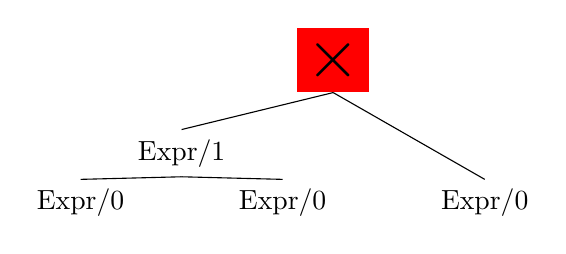
\begin{tikzpicture}
		\tikzset{level 1+/.style={level distance=15\baselineskip}}
		\tikzset{level 1+/.style={sibling distance=2.9\baselineskip}}
		\tikzset{frontier/.style={distance from root=4\baselineskip}}
		\Tree [.\node[fill=red]{\Huge$\times$}; [.Expr/1 Expr/0 Expr/0 ] Expr/0 ]
	\end{tikzpicture}
\end{center}
\end{frame}

\begin{frame}
\frametitle{Grammar rules levels}
\small
\begin{center}
\texttt{(R2:[ Expression/1 -> Expression/0 lexAdd Expression/1 ])}
\end{center}
\begin{center}
	\large
	\begin{tikzpicture}
		\tikzset{level 1+/.style={level distance=15\baselineskip}}
		\tikzset{level 1+/.style={sibling distance=2.9\baselineskip}}
		\tikzset{frontier/.style={distance from root=4\baselineskip}}
		\Tree [.\node[color=fg!0]{Expr/1}; \edge[color=fg!0]; Expr/0 \edge[color=fg!0]; [.\node[color=fg!0]{Expr/1}; \edge[color=fg!0]; Expr/0 \edge[color=fg!0]; Expr/0 ] ]
	\end{tikzpicture}
\end{center}
\end{frame}

\begin{frame}[noframenumbering]
\frametitle{Grammar rules levels}
\small
\begin{center}
\texttt{(R2:[ Expression/1 -> Expression/0 lexAdd Expression/1 ])}
\end{center}
\begin{center}
	\large
	\begin{tikzpicture}
		\tikzset{level 1+/.style={level distance=15\baselineskip}}
		\tikzset{level 1+/.style={sibling distance=2.9\baselineskip}}
		\tikzset{frontier/.style={distance from root=4\baselineskip}}
		\Tree [.\node[color=fg!0]{Expr/1}; \edge[color=fg!0]; Expr/0 \edge[color=fg!0]; [.Expr/1 Expr/0 Expr/0 ] ]
	\end{tikzpicture}
\end{center}
\end{frame}

\begin{frame}[noframenumbering]
\frametitle{Grammar rules levels}
\small
\begin{center}
\texttt{(R2:[ Expression/1 -> Expression/0 lexAdd Expression/1 ])}
\end{center}
\begin{center}
	\large
	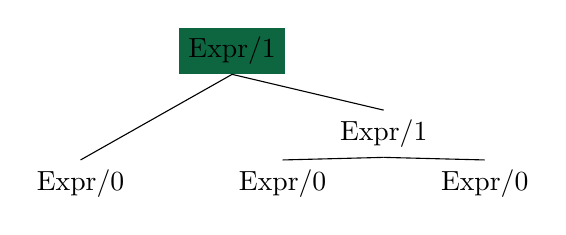
\begin{tikzpicture}
		\tikzset{level 1+/.style={level distance=15\baselineskip}}
		\tikzset{level 1+/.style={sibling distance=2.9\baselineskip}}
		\tikzset{frontier/.style={distance from root=4\baselineskip}}
		\Tree [.\node[fill=green]{Expr/1}; Expr/0 [.Expr/1 Expr/0 Expr/0 ] ]
	\end{tikzpicture}
\end{center}
\end{frame}

\begin{frame}[fragile]
\frametitle{Lekta dialogue manager structure}
\begin{center}
	\large
	\begin{tikzpicture}[level distance=50pt]
		\tikzset{level 1+/.style={level distance=20\baselineskip}}
		\tikzset{level 1+/.style={sibling distance=1.9\baselineskip}}
		\Tree [.Cogito \edge[very thick,<-,>=latex,green]; [.Senso \edge[very thick,<-,>=latex,green]; [.Colligo \edge[very thick,<-,>=latex,green]; NLU \edge[color=fg!0]; \node[color=fg!0]{A}; ] \edge[color=fg!0]; \edge[color=fg!0]; \node[color=fg!0]{A}; ] \edge[very thick,->,>=latex,green]; [.Respondo \edge[color=fg!0]; \node[color=fg!0]{A}; \edge[very thick,->,>=latex,green]; [.Locutio \edge[color=fg!0]; \node[color=fg!0]{A}; \edge[very thick,->,>=latex,green]; {Scribo (NLG)} ] ] ]
	\end{tikzpicture}
\end{center}
\end{frame}

\begin{frame}[fragile]
\frametitle{NLU: Natural Language Understanding}
\begin{itemize}
	\item Its	main objective is to convert user proference in two or more root types (defined in \texttt{setupParserRoots}).
	\item For example ``\texttt{Expression}'' if we want a mathematical expressions parser.
	\item Uses defined lexicon and grammar rules.
	\item All previous examples and exercises are included in this stage.
\end{itemize}
\begin{center}
	\tiny
	\begin{tikzpicture}[level distance=25pt]
		\tikzset{level 1+/.style={level distance=20\baselineskip}}
		\tikzset{level 1+/.style={sibling distance=1.9\baselineskip}}
		\Tree [.Cogito \edge[very thick,<-,>=latex,green]; [.Senso \edge[very thick,<-,>=latex,green]; [.Colligo \edge[very thick,<-,>=latex,green]; \node[fill=red]{NLU}; \edge[color=fg!0]; \node[color=fg!0]{A}; ] \edge[color=fg!0]; \edge[color=fg!0]; \node[color=fg!0]{A}; ] \edge[very thick,->,>=latex,green]; [.Respondo \edge[color=fg!0]; \node[color=fg!0]{A}; \edge[very thick,->,>=latex,green]; [.Locutio \edge[color=fg!0]; \node[color=fg!0]{A}; \edge[very thick,->,>=latex,green]; {Scribo (NLG)} ] ] ]
	\end{tikzpicture}
\end{center}
\end{frame}

\begin{frame}[fragile]
\frametitle{Colligo: From \emph{latin}, to gather}
\begin{itemize}
	\item It can be used to join two or more parser roots.
	\item For example: Two consecutives greetings can be merged into only one (\texttt{U: Hello, good morning! ...}).
	\item Possibly in the future this stage will be transformed in some high-level grammar scheme.
\end{itemize}
\begin{center}
	\tiny
	\begin{tikzpicture}[level distance=25pt]
		\tikzset{level 1+/.style={level distance=20\baselineskip}}
		\tikzset{level 1+/.style={sibling distance=1.9\baselineskip}}
		\Tree [.Cogito \edge[very thick,<-,>=latex,green]; [.Senso \edge[very thick,<-,>=latex,green]; [.\node[fill=red]{Colligo}; \edge[very thick,<-,>=latex,green]; NLU \edge[color=fg!0]; \node[color=fg!0]{A}; ] \edge[color=fg!0]; \edge[color=fg!0]; \node[color=fg!0]{A}; ] \edge[very thick,->,>=latex,green]; [.Respondo \edge[color=fg!0]; \node[color=fg!0]{A}; \edge[very thick,->,>=latex,green]; [.Locutio \edge[color=fg!0]; \node[color=fg!0]{A}; \edge[very thick,->,>=latex,green]; {Scribo (NLG)} ] ] ]
	\end{tikzpicture}
\end{center}
\end{frame}

\begin{frame}[fragile]
\frametitle{Colligo: From \emph{latin}, to gather}
\setbeamercolor{block title}{use=structure,fg=white,bg=red!75!black}
\setbeamercolor{block body}{use=structure,fg=black,bg=red!10!white}
\begin{block}{Colligo rules template: \texttt{ColligoSchemata} section}
\scriptsize
\begin{lstlisting}[language=lekta]
(ColligoScheme <rule_name> : [ in_1 ... in_n >> output ]
	ColligoCapture {
		// Preconditions 
		<condition_1> &&
		<condition_2> &&
		...
	}
 	ColligoAction {
		// Actions to be executed when triggered
		<command_1>;
		<command_2>;
		...
		// ^OBJSENSO stands for output term.
		// #OBJCOLLIGO-1 stands for first input term.
		// #OBJCOLLIGO-2 stands for second input term.
		// #OBJCOLLIGO-N stands for nth input term.
	}
)
\end{lstlisting}
\end{block}
\end{frame}

\begin{frame}[fragile]
\frametitle{Senso: From \emph{latin}, to sense, to feel}
\begin{itemize}
	\item It corresponds to the sensory part of the use of language.
	\item Used to filter useless proferences to the dialogue manager.
	\item Usually this stage writes non-filtered user proferences directly into ``mindboard''.
	\item So we can use some rule of this stage to initialize context and mind structures.
\end{itemize}
\begin{center}
	\tiny
	\begin{tikzpicture}[level distance=25pt]
		\tikzset{level 1+/.style={level distance=20\baselineskip}}
		\tikzset{level 1+/.style={sibling distance=1.9\baselineskip}}
		\Tree [.Cogito \edge[very thick,<-,>=latex,green]; [.\node[fill=red]{Senso}; \edge[very thick,<-,>=latex,green]; [.Colligo \edge[very thick,<-,>=latex,green]; NLU \edge[color=fg!0]; \node[color=fg!0]{A}; ] \edge[color=fg!0]; \edge[color=fg!0]; \node[color=fg!0]{A}; ] \edge[very thick,->,>=latex,green]; [.Respondo \edge[color=fg!0]; \node[color=fg!0]{A}; \edge[very thick,->,>=latex,green]; [.Locutio \edge[color=fg!0]; \node[color=fg!0]{A}; \edge[very thick,->,>=latex,green]; {Scribo (NLG)} ] ] ]
	\end{tikzpicture}
\end{center}
\end{frame}

\begin{frame}[fragile]
\frametitle{Senso: From \emph{latin}, to sense, to feel}
\setbeamercolor{block title}{use=structure,fg=white,bg=red!75!black}
\setbeamercolor{block body}{use=structure,fg=black,bg=red!10!white}
\begin{block}{Senso rules template: \texttt{SensoSchemata} section}
\scriptsize
\begin{lstlisting}[language=lekta]
(SensoScheme <rule_name> : [ in_1 ... in_n ]
	SensoCapture {
		// Preconditions 
		<condition_1> &&
		<condition_2> &&
		...
	}
 	SensoAction {
		// Actions to be executed when triggered
		<command_1>;
		<command_2>;
		...
		// #OBJSENSO-1 stands for first input term.
		// #OBJSENSO-2 stands for second input term.
		// #OBJSENSO-N stands for nth input term.
	}
)
\end{lstlisting}
\end{block}
\end{frame}

\begin{frame}[fragile]
\frametitle{Cogito: From \emph{latin}, to think}
\begin{itemize}
	\item Its the module that simulates human thinking, context-dependant pragmatics, and logic reasoning.
	\item It uses some global data structures (the only ones in Lekta) that any other module can read and even write.
\end{itemize}
\begin{center}
	\tiny
	\begin{tikzpicture}[level distance=25pt]
		\tikzset{level 1+/.style={level distance=20\baselineskip}}
		\tikzset{level 1+/.style={sibling distance=1.9\baselineskip}}
		\Tree [.\node[fill=red]{Cogito}; \edge[very thick,<-,>=latex,green]; [.Senso \edge[very thick,<-,>=latex,green]; [.Colligo \edge[very thick,<-,>=latex,green]; NLU \edge[color=fg!0]; \node[color=fg!0]{A}; ] \edge[color=fg!0]; \edge[color=fg!0]; \node[color=fg!0]{A}; ] \edge[very thick,->,>=latex,green]; [.Respondo \edge[color=fg!0]; \node[color=fg!0]{A}; \edge[very thick,->,>=latex,green]; [.Locutio \edge[color=fg!0]; \node[color=fg!0]{A}; \edge[very thick,->,>=latex,green]; {Scribo (NLG)} ] ] ]
	\end{tikzpicture}
\end{center}
\end{frame}

\begin{frame}[fragile]
\frametitle{Cogito: From \emph{latin}, to think}
\setbeamercolor{block title}{use=structure,fg=white,bg=red!75!black}
\setbeamercolor{block body}{use=structure,fg=black,bg=red!10!white}
\begin{block}{Mindboard structures definition: \texttt{conversationalModel} section}
\scriptsize
\begin{lstlisting}[language=lekta]
MindBoardStructure: {
	( <name_of_field_1> / <field_type_1> )
	...
	( <name_of_field_n> / <field_type_n> )
}
\end{lstlisting}
\end{block}
\setbeamercolor{block title}{use=structure,fg=white,bg=green!75!black}
\setbeamercolor{block body}{use=structure,fg=black,bg=green!10!white}
\begin{block}{Mindboard structures example}
\scriptsize
\begin{lstlisting}[language=lekta]
MindBoardStructure: {
	( Counter / integer )
	( Error / bool )
}
...
// To access these fields:
$MINDBOARD@Counter <- 0;
$MINDBOARD@Error <- False;
\end{lstlisting}
\end{block}
\end{frame}

\begin{frame}[fragile]
\frametitle{Cogito: From \emph{latin}, to think}
\setbeamercolor{block title}{use=structure,fg=white,bg=red!75!black}
\setbeamercolor{block body}{use=structure,fg=black,bg=red!10!white}
\begin{block}{Cogito rules template: \texttt{CogitoSchemata} section}
\scriptsize
\begin{lstlisting}[language=lekta]
(CogitoScheme <rule_name> : 
	CogitoCapture {
		// Preconditions 
		<condition_1> &&
		<condition_2> &&
		...
	}
 	CogitoAction {
		// Actions to be executed when triggered
		<command_1>;
		<command_2>;
		...
		// Some useful built-in functions here could be :
		// CogitoQuit(): Stop processing cogito rules.
		// CogitoRetry(): Restart processing cogito rules.
	}
)
\end{lstlisting}
\end{block}
\end{frame}

\begin{frame}[fragile]
\frametitle{Respondo: From \emph{latin}, to answer}
\begin{itemize}
	\item It corresponds to the motor part of the use of language.
	\item It can be used to split what system wants to say in some individual parts easier to generate.
\end{itemize}
\begin{center}
	\tiny
	\begin{tikzpicture}[level distance=25pt]
		\tikzset{level 1+/.style={level distance=20\baselineskip}}
		\tikzset{level 1+/.style={sibling distance=1.9\baselineskip}}
		\Tree [.Cogito \edge[very thick,<-,>=latex,green]; [.Senso \edge[very thick,<-,>=latex,green]; [.Colligo \edge[very thick,<-,>=latex,green]; NLU \edge[color=fg!0]; \node[color=fg!0]{A}; ] \edge[color=fg!0]; \edge[color=fg!0]; \node[color=fg!0]{A}; ] \edge[very thick,->,>=latex,green]; [.\node[fill=red]{Respondo}; \edge[color=fg!0]; \node[color=fg!0]{A}; \edge[very thick,->,>=latex,green]; [.Locutio \edge[color=fg!0]; \node[color=fg!0]{A}; \edge[very thick,->,>=latex,green]; {Scribo (NLG)} ] ] ]
	\end{tikzpicture}
\end{center}
\end{frame}

\begin{frame}[fragile]
\frametitle{Respondo: From \emph{latin}, to answer}
\setbeamercolor{block title}{use=structure,fg=white,bg=red!75!black}
\setbeamercolor{block body}{use=structure,fg=black,bg=red!10!white}
\begin{block}{Respondo rules template: \texttt{RespondoSchemata} section}
\scriptsize
\begin{lstlisting}[language=lekta]
(RespondoScheme <rule_name> : [ output ]
	RespondoCapture {
		// Preconditions 
		<condition_1> &&
		<condition_2> &&
		...
	}
 	RespondoAction {
		// Actions to be executed when triggered
		<command_1>;
		<command_2>;
		...
		// ^OBJRESPONDO stands for output expression.
	}
)
\end{lstlisting}
\end{block}
\end{frame}

\begin{frame}[fragile]
\frametitle{Locutio: From \emph{latin}, to speak}
\begin{itemize}
	\item It may be used to sort expressions given by \texttt{Respondo} module in order to make the dialogue more natural.
	\item For example, if we want to say lots of thing, some of them (for example questions) should be put at the end of the dialogue act.
\end{itemize}
\begin{center}
	\tiny
	\begin{tikzpicture}[level distance=25pt]
		\tikzset{level 1+/.style={level distance=20\baselineskip}}
		\tikzset{level 1+/.style={sibling distance=1.9\baselineskip}}
		\Tree [.Cogito \edge[very thick,<-,>=latex,green]; [.Senso \edge[very thick,<-,>=latex,green]; [.Colligo \edge[very thick,<-,>=latex,green]; NLU \edge[color=fg!0]; \node[color=fg!0]{A}; ] \edge[color=fg!0]; \edge[color=fg!0]; \node[color=fg!0]{A}; ] \edge[very thick,->,>=latex,green]; [.Respondo \edge[color=fg!0]; \node[color=fg!0]{A}; \edge[very thick,->,>=latex,green]; [.\node[fill=red]{Locutio}; \edge[color=fg!0]; \node[color=fg!0]{A}; \edge[very thick,->,>=latex,green]; {Scribo (NLG)} ] ] ]
	\end{tikzpicture}
\end{center}
\end{frame}

\begin{frame}[fragile]
\frametitle{Locutio: From \emph{latin}, to speak}
\setbeamercolor{block title}{use=structure,fg=white,bg=red!75!black}
\setbeamercolor{block body}{use=structure,fg=black,bg=red!10!white}
\begin{block}{Locutio rules template: \texttt{LocutioSchemata} section}
\scriptsize
\begin{lstlisting}[language=lekta]
(LocutioScheme <rule_name> : [ in_1 ... in_n >> output ]
	LocutioCapture {
		// Preconditions 
		<condition_1> &&
		<condition_2> &&
		...
	}
 	LocutioAction {
		// Actions to be executed when triggered
		<command_1>;
		<command_2>;
		...
		// ^OBJLOCUTIO stands for output expression.
		// #OBJRESPONDO-1 stands for first input term.
		// #OBJRESPONDO-2 stands for second input term.
		// #OBJRESPONDO-N stands for nth input term.
	}
)
\end{lstlisting}
\end{block}
\end{frame}

\begin{frame}[fragile]
\frametitle{Scribo: From \emph{latin}, to write}
\begin{itemize}
	\item It's used to generate system proferences into target natural language.
	\item So it's a language dependant module (as well as lexicon and grammar ones).
	\item Related section in main project file: \texttt{scriboModel forLanguage <...>}.
\end{itemize}
\begin{center}
	\tiny
	\begin{tikzpicture}[level distance=25pt]
		\tikzset{level 1+/.style={level distance=20\baselineskip}}
		\tikzset{level 1+/.style={sibling distance=1.9\baselineskip}}
		\Tree [.Cogito \edge[very thick,<-,>=latex,green]; [.Senso \edge[very thick,<-,>=latex,green]; [.Colligo \edge[very thick,<-,>=latex,green]; NLU \edge[color=fg!0]; \node[color=fg!0]{A}; ] \edge[color=fg!0]; \edge[color=fg!0]; \node[color=fg!0]{A}; ] \edge[very thick,->,>=latex,green]; [.Respondo \edge[color=fg!0]; \node[color=fg!0]{A}; \edge[very thick,->,>=latex,green]; [.Locutio \edge[color=fg!0]; \node[color=fg!0]{A}; \edge[very thick,->,>=latex,green]; \node[fill=red]{Scribo (NLG)}; ] ] ]
	\end{tikzpicture}
\end{center}
\end{frame}

\begin{frame}[fragile]
\frametitle{Scribo: From \emph{latin}, to write}
\setbeamercolor{block title}{use=structure,fg=white,bg=red!75!black}
\setbeamercolor{block body}{use=structure,fg=black,bg=red!10!white}
\begin{block}{Scribo rules template: \texttt{ScriboSchemata} subsection}
\scriptsize
\begin{lstlisting}[language=lekta]
(ScriboScheme <rule_name> : [ in_1 ... in_n ]
	ScriboCapture {
		// Preconditions 
		<condition_1> &&
		<condition_2> &&
		...
	}
 	ScriboAction {
		// Actions to be executed when triggered
		<command_1>;
		<command_2>;
		...
		// #OBJLOCUTIO-1 stands for first input term.
		// #OBJLOCUTIO-2 stands for second input term.
		// #OBJLOCUTIO-N stands for nth input term.
	}
)
\end{lstlisting}
\end{block}
\end{frame}

\begin{frame}[fragile]
\frametitle{Scribo: From \emph{latin}, to write}
Two useful built-in functions here:
\begin{itemize}
	\item \texttt{SetMainAnswerString(string s):} Generates system answer in accumulative way.
	\item \texttt{SetMainAnswerStringRandom(string s1, string s2, ...):} Chooses an answer randomly between its arguments.
\end{itemize}
\setbeamercolor{block title}{use=structure,fg=white,bg=green!75!black}
\setbeamercolor{block body}{use=structure,fg=black,bg=green!10!white}
\begin{block}{Example}
\tiny
\begin{lstlisting}[language=lekta]
string greet;
cond {
	(ClockAskHour() < 7)  greet <- 'Good night. ';
	(ClockAskHour() < 14) greet <- 'Good morning. ';
	(ClockAskHour() < 20) greet <- 'Good afternoon. ';
	default               greet <- 'Good night. ';
}
SetMainAnswerString( greet );
SetMainAnswerStringRandom( 
		'Welcome to the Personal Assistant Service. ',
		'Thanks for contacting the Personal Assistant Service. ',
		'Your Personal Assistant Service speaking. ',
		'Thank you for calling the Personal Assistant Service. ');
\end{lstlisting}
\end{block}
\end{frame}

\begin{frame}[fragile]
\Huge
\begin{center}
Session 04: Exercise 01\\
Dialogue system: Integer calculator
\end{center}
\end{frame}

\subsection{Exercise 02}

\begin{frame}[fragile]
\frametitle{Metatype StructureBatch}
\begin{itemize}
	\item Used to create sequences of some type.
	\item They are similar to dequeues (you can insert and remove elements in both ends). By the way, positions start in 1.
	\item But you can also ``read'' and ``write'' elements in other positions.
\end{itemize}
\setbeamercolor{block title}{use=structure,fg=white,bg=green!75!black}
\setbeamercolor{block body}{use=structure,fg=black,bg=green!10!white}
\begin{block}{Example}
\scriptsize
\begin{lstlisting}[language=lekta]
classDef:ElementInt( integer )
classDef:StructureBatch( Counters: ( integer ) )
...
Counters counters;
Counter c1 <- 1;
Counter c2 <- 2;
Counter c3 <- 3;

BatchInsertEnd(counters, c1);
BatchInsertEnd(counters, c2);
BatchInsertEnd(counters, c3); // {c1, c2, c3}
\end{lstlisting}
\end{block}
\end{frame}

\begin{frame}[fragile]
\frametitle{Metatype StructureBatch}
\setbeamercolor{block title}{use=structure,fg=white,bg=green!75!black}
\setbeamercolor{block body}{use=structure,fg=black,bg=green!10!white}
\begin{block}{Batch built-in functions}
\scriptsize
\begin{lstlisting}[language=lekta]
integer BatchSize(batch b);
batch BatchJoin(batch b1, batch b2);

procedure BatchExtractInit(batch b, elem out);
procedure BatchExtractEnd(batch b, elem out);
procedure BatchInsertInit(batch, elem in);
procedure BatchInsertEnd(batch b, elem in);

procedure BatchRecoverPosition
          (batch b, integer pos, elem out);
procedure BatchAssignPosition
          (batch b, integer pos, elem in);

procedure BatchExchange
          (batch b, integer pos1, integer pos2);
\end{lstlisting}
\end{block}
\end{frame}

\begin{frame}[fragile]
\Huge
\begin{center}
Session 04: Exercise 02\\
Dialogue system: Basic domotic assistant
\end{center}
\end{frame}

\end{document}

